在这一节,我们对上述绍四种 Attention 加速方法的性能进行衡量。我们采用~\cite{tay2021long}中提出的 Long Range Arena 基准比较各方法的建模能力和运行开销。最后,我们也探索了MEGA模型在的部分超参对模型性能的影响。
\subs{实现细节}
\subsubs{数据集}
Long Range Arena 数据集~\cite{tay2021long} 被广泛用于验证模型的长序列建模性能,其从不同角度设计了5种序列建模任务。

文本序列分类任务(Text)。任务采用 IMDB 数据集,输入为字节级表示(而非事先分词)文本,要求模型输出为文本情感的二分类。最大上下文长度为 4K。

结构化操作任务(ListOps)。这一任务测量模型对结构化长序列的建模能力,其输入为一段嵌套的操作序列,要求模型输出操作的结果(输出为0至9,建模为10分类任务),其最长上下文长度为 2K。下面举一个例子对任务进行说明

\begin{verbatim}
    输入 [ MAX 4 3 [ MIN 2 3 ] 1 0 [ MEDIAN 1 5 8 9 2] ]
    输出 5
\end{verbatim}
    
文本序列检索任务(Retrieval)。这一任务要求模型分别将两段文本分别压缩为两个向量,接下来再由着两个向量的相关性判断这两段文本是否相关。对每段文本,限制上下文长度为 4K,因此上下文长度的总上限为 8K。

图像分类任务(Image)。这一任务将 CIFAR-10 数据集形状为 $N\times N$ 的图像首先转换为 8 位的灰度图,接下来展开成 $N^2$ 的序列直接输入模型,要求模型给出十分类结果。这一任务衡量模型对序列复杂信息的建模能力,即能否在没有二维先验的情形下准备把握线性输入中的二维信息。CIFAR-10 中的图像大小为 $32\times 32$,因此该任务的输入长度为 1K。

图像分析任务(Pathfinder)。这一任务给模型呈现一幅灰度图像,要求模型找出图像中的两个点是否可以被图中的线所连接。该任务有 2 个版本,Pathfinder 和 Pathfiner-X,前者将图像降采样到 $32\times 32$ 后展开为一个长度为 1K 的序列输入模型,而后者则降采样到 $128\times 128$,输入序列长达 16K。Pathfinder-X 序列长,且输入无二维先验,训练时间和算力开销相当大,因此本文仅使用 1K 序列长度的版本进行测试。

值得注意的是,不同模型对图像输入序列的处理方式有很大差异。Skyformer, CosFormer 和 LARA 在模型实现时将 $0\sim 255$ 分别映射到一个随机初始化的向量中,所有 $256$ 个向量的表征自行学习,不加约束。而 MEGA 的处理方式则引入了一个线性变化的先验。具体来说是引入可学习的向量 $w$ 和 $b$,再将输入归一化到 $[-\frac 1 2, \frac 1 2]$,由此将归一化的输入 $x$ 嵌入到向量 $v(x)=xw+b$。实验中,我们发现后者的训练难度要比前者更高,容易出现模型不收敛,甚至损失函数值在长达 50k 次梯度更新的训练过程中纹丝不动的情况。在与~\cite{ma2023mega}的作者联系后,我们使用指数预热的方式使训练过程可以较为稳定地收敛。

% Table generated by Excel2LaTeX from sheet 'Results'
\begin{table}[htbp]
  \centering

  \caption{实验中所用模型的参数量 ($\times 10^5$)}
    \begin{tabular}{c|ccccc}
    \hline
    Model & Text  & ListOps & Retrieval & Pathfinder & Image \bigstrut\\
    \hline
    Baseline & 37.06  & 20.98  & 39.51  & 17.40  & 15.86  \bigstrut[t]\\
    CosFormer & 37.06  & 20.98  & 39.51  & 17.40  & 15.86  \\
    LARA  & 42.10  & 26.02  & 44.56  & 22.44  & 20.90  \\
    Skyformer & 37.06  & 20.98  & 39.51  & 17.40  & 15.86  \bigstrut[b]\\
    \hline
    MEGA-128 & 94.78  & 58.02  & 137.61  & 137.61  & 282.48  \bigstrut[t]\\
    MEGA-$\infty$ & 97.88  & 60.27  & 146.52  & 138.69  & 283.91  \bigstrut[b]\\
    \hline
    \end{tabular}%
  \label{tab:model_size}
\end{table}%


\subsubs{模型和训练参数}
本节的实验共涉及 6 种模型的对比。其中 Baseline 表示未经优化的原始 Softmax Attention 实现, CosFormer,LARA,Skyformer 和 MEGA 是前述的 4 种方法。其中 MEGA-$\infty$ 表示未经块划分的 MEGA 实现,而 MEGA-128 表示分块长度 $c=128$ 的 MEGA 实现。

我们选取了2种不同的配置。第一组实验(下称 Setting-1),包括 Baseline,CosFormer,LARA 和 Skyformer,模型规格与超参数跟随Skyformer~\cite{chen2021skyformer}第 5 节的设定 。第二组实验(下称 Setting-2),包括 MEGA-128 和 MEGA-$\infty$,模型规格和超参数跟随~\cite{ma2023mega}的设定,详见~\cite{ma2023mega}的附录 D.1。对于模型的参数量,我们在表~\ref{tab:model_size}中进行了列举。就训练平台来说,我们在单张 NVIDIA RTX-3090 上进行CosFormer,LARA 和 Skyformer 的训练,而由于 MEGA 在其论文所指定的模型规模对显存要求较高,因此我们在 NVIDIA A100-SXM4-80GB 集群上进行MEGA的训练。推理时,两组实验的所有模型都在单张 NVIDIA A100-SXM4-80GB 上运行,batch 大小均与第一组实验的训练 batch 大小一致。


\subs{建模能力}
\label{subsec:lra_perf}

% Table generated by Excel2LaTeX from sheet 'Results'
\begin{table}[htbp]
  \centering
  \caption{不同计算方法在 Long Range Arena 基准的表现}
    \begin{tabular}{c|c|cccccc}
    \hline
          & Model & Text  & ListOps & Retrieval & Pathfinder & Image & Average \bigstrut\\
    \hline
    \multirow{6}[4]{*}{Reported} & Baseline & 61.95  & 38.37  & 80.69  & 65.26  & 40.57  & 57.37  \bigstrut[t]\\
          & CosFormer & 63.41  & 37.90  & 61.36  & 70.33  & \underline{43.17} & 55.23  \\
          & LARA  & \underline{64.77} & \underline{39.21} & 81.18  & \underline{72.02} & 38.40  & 59.12  \\
          & Skyformer & 64.70  & 38.69  & \underline{82.06} & 70.73  & 40.77  & \underline{59.39} \bigstrut[b]\\
\cline{2-8}          & MEGA-128 & 90.19  & 58.76  & 90.97  & 94.41  & 85.80  & 84.03  \bigstrut[t]\\
          & MEGA-$\infty$ & \underline{90.43} & \underline{63.14} & \underline{91.25} & \underline{96.01} & \underline{90.44} & \underline{86.25} \bigstrut[b]\\
    \hline
    \multirow{5}[4]{*}{Reproduced} & CosFormer & 63.70  & 38.91  & 80.94  & \underline{74.22} & \underline{39.69} & \underline{59.49} \bigstrut[t]\\
          & LARA  & \underline{64.26} & 37.20  & 80.27  & 66.69  & 36.49  & 56.98  \\
          & Skyfomer & 60.60  & \underline{39.57} & \underline{81.76} & 68.76  & 32.52  & 56.64  \bigstrut[b]\\
\cline{2-8}          & MEGA-128 & 89.78  & 57.55  & 90.84  & 94.62  & 86.14  & 83.79  \bigstrut[t]\\
          & MEGA-$\infty$ & \underline{90.20} & \underline{64.20} & \underline{91.07} & \underline{95.75} & \underline{89.78} & \underline{86.20} \bigstrut[b]\\
    \hline
    \end{tabular}%
  \label{tab:lra_main}%
\end{table}%


表~\ref{tab:lra_main}列举了不同模型的在 Long Range Arena 上的表现。其中 Reported 为每种算法在论文中汇报的实验结果, Reproduced 为我们实际训练后得到的实验结果。

Setting-1 中实验在 Image 任务上的性能与论文汇报有较为明显的差距。在进行了一定的模型尺寸和超参数搜索后,我们也可以得到一个与论文汇报结果类似的值,但是模型的参数量出现了显著提高。考虑到参数量,训练步数的比较公平性,我们在这里呈现依照论文中参数得到的训练结果。

在复现结果的 Setting-1 中,CosFormer 在图像处理任务 Image 和 Pathfinder 中的表现较为突出,这主要得益于Cosformer关注了softmax注意力矩阵的非负性和非线性重加权机制,余弦重加权有助于模型放大局部相关性,这一点相比于其他方法能更好地关注图像像素点间的相关性以及局部特征。

而在 Setting-2 中,感受野一定程度上受限的 MEGA-128 在结构化处理任务 ListOps 上与不受限的 MEGA-$\infty$ 差异较大,而在其他 4 个任务中差异较小。ListOps 任务的完成需要模型对序列中每个元素的位置,所归属的操作,以及所在的嵌套深度都充分的理解,而 MEGA-128 需要逐层积累的感受野可能限制了模型对远距离相关性的学习速度,而实验中采用模型的层数较少,从而显著降低了性能。

\subs{训练与推理开销}

表 ~\ref{tab:training} 和表 ~\ref{tab:inference} 分别列举了模型在训练和推理过程中开销,其中“训练”指在训练集中训练1轮,而“推理”是指在相应任务的测试集中推理1轮。训练集和测试集的划分遵循~\cite{tay2021long}的设定。表中 PeakMemory 表示训练/推理过程中显存占用的最大值,单位为 GB;而 Time 表示相应操作的用时,单位为秒。

在 Setting-1 中,Baseline 相比各种优化算法显著消耗了更多的时间和显存。而在各类优化方法中,LARA的优化效果最为显著,对于长序列(Text,上下文长度最大4K)在训练和推理时的加速比可达3.89和4.11。这主要得益于LARA同时结合了RFA和RA的优点,利用多重重要性采样,在很好地近似了softmax attention的同时,实现了线性的时间及空间复杂度,是一种极其有效的方法。 而 CosFormer 和 Skyformer 的加速效果则在长序列任务,如Text和Retrieval 中较为显著;对于仅有 1K 上下文的 Pathfinder 和 Retrieval,Skyformer 与 Baseline 耗时基本相当,而 CosFormer 甚至不如 Baseline。这可能表明 SkyFormer 和 CosFormer 的加速主要适用于长序列。另一种可能得原因是 SkyFormer 和 CosFormer 的实现较为朴素,其对 batch 的支持不佳(Pathfinder 和 Image 在训练时的的 batch 大小分别为 128 和 256),致使其未能充分开发 batch 级别的并行性。

在 Setting-2 中,MEGA-128 比 MEGA-$\infty$ 显著提高了推理和训练速度,并节约了显存占用。在 Text 和 Retrieval 任务中,尽管 MEGA-128 的参数量分别为Setting-1 中 Baseline的2.6倍和3.5倍,但 MEGA-128 仍然比 Baseline 有更好快的速度和更少的显存用量。Setting-2 的实验表明, MEGA-chunk 在 Attention 加速计算上,相比 MEGA-$\infty$和普通的Attention都是十分高效的。

值得指出的是,算法性能的测量结果不仅取决于算法的理论复杂度,更深受代码实现效率的影响。一个较为极端的例子是我们曾试图复现的 Diffuser~\cite{feng2023diffuser},其算法本身看起来加速效果显著,然而当 batch 非常大时,其实现依赖的 \verb|dgl| 计算速度相比 \verb|torch| 的注意力实现效率低得多,使其训练速度慢到了几乎无法接受的程度。

% Table generated by Excel2LaTeX from sheet 'Results'
\begin{table}[htbp]
  \centering

  \caption{不同计算方式的训练开销}
    \begin{tabular}{c|c|ccccc}
    \hline
          & Model & Text  & ListOps & Retrieval & Pathfinder & Image \bigstrut\\
    \hline
    \multicolumn{1}{c|}{\multirow{6}[4]{*}{Peak\newline{}Memory(GB) ($\downarrow$)}} & Baseline & 20.74  & 5.37  & 10.77  & 5.73  & 11.47  \bigstrut[t]\\
          & CosFormer & 9.05  & 4.53  & 7.15  & 9.05  & 18.09  \\
          & LARA  & \underline{1.90} & \underline{0.95} & \underline{1.82} & \underline{1.92} & \underline{3.80} \\
          & Skyformer & 3.18  & 1.75  & 3.15  & 4.13  & 8.25  \bigstrut[b]\\
\cline{2-7}          & MEGA-128 & \underline{14.86} & \underline{9.03} & \underline{55.69} & \underline{13.97} & \underline{9.31} \bigstrut[t]\\
          & Mega-$\infty$ & 45.19  & 21.98  & -     & 21.03  & 12.67  \bigstrut[b]\\
    \hline
    \multirow{6}[4]{*}{Time(s) ($\downarrow$)} & Baseline & 181.63 & 214.19 & 2117.04 & 114.22 & 31.22 \bigstrut[t]\\
          & CosFormer & 104.3 & 209.24 & 1362.41 & 159.71 & 43.86 \\
          & LARA  & \underline{46.71} & \underline{101.07} & \underline{569.74} & \underline{76.49} & \underline{20.48} \\
          & Skyformer & 60.16 & 136.18 & 761.11 & 106.64 & 28.76 \bigstrut[b]\\
\cline{2-7}          & MEGA-128 & \underline{72.79} & \underline{248.14} & \underline{1195.85} & \underline{173.92} & \underline{95.97} \bigstrut[t]\\
          & MEGA-$\infty$ & 234.89  & 448.02  & -     & 255.54  & 129.67  \bigstrut[b]\\
    \hline
    \end{tabular}%
   \label{tab:training}
\end{table}%


% Table generated by Excel2LaTeX from sheet 'Results'
\begin{table}[htbp]
  \centering
  \caption{不同计算方式的推理开销}
    \begin{tabular}{c|c|ccccc}
    \hline
          & Model & Text  & ListOps & Retrieval & Pathfinder & Image \bigstrut\\
    \hline
    \multicolumn{1}{c|}{\multirow{6}[4]{*}{PeakMemory(GB) ($\downarrow$)}} & Baseline & 8.27  & 2.14  & 4.16  & 2.27  & 4.54  \bigstrut[t]\\
          & CosFormer & 4.56  & 2.28  & 2.30  & 4.55  & 9.10  \\
          & LARA  & \underline{0.78} & \underline{0.39} & \underline{0.40} & \underline{0.78} & \underline{1.54} \\
          & Skyformer & 1.12  & 0.56  & 0.58  & 1.12  & 2.24  \bigstrut[b]\\
\cline{2-7}          & MEGA-128 & \underline{4.13} & \underline{3.59} & \underline{2.66} & \underline{5.53} & \underline{0.73} \bigstrut[t]\\
          & MEGA-$\infty$ & 14.71  & 9.98  & 9.49  & 11.54  & 1.29  \bigstrut[b]\\
    \hline
    \multirow{6}[4]{*}{Time(s) ($\downarrow$)} & Baseline & 43.01 & 0.99  & 58.3  & 3.28  & 1.55 \bigstrut[t]\\
          & CosFormer & 23.65 & 0.98  & 41.12 & 4.46  & 2.15 \\
          & LARA  & \underline{10.46} & \underline{0.47} & \underline{15.4} & \underline{2.34} & \underline{1.14} \\
          & Skyformer & 13.86 & 0.69  & 21.95 & 3.27  & 1.54 \bigstrut[b]\\
\cline{2-7}          & MEGA-128 & \underline{22.89} & \underline{1.13} & \underline{47.55} & \underline{7.83} & \underline{6.55} \bigstrut[t]\\
          & Mega-$\infty$ & 94.52  & 2.96  & 159.36  & 12.32  & 9.66  \bigstrut[b]\\
    \hline
    \end{tabular}%
  \label{tab:inference}%
\end{table}%


\begin{figure}[htbp]
\centering

\begin{subfigure}[b]{0.45\textwidth}
\centering
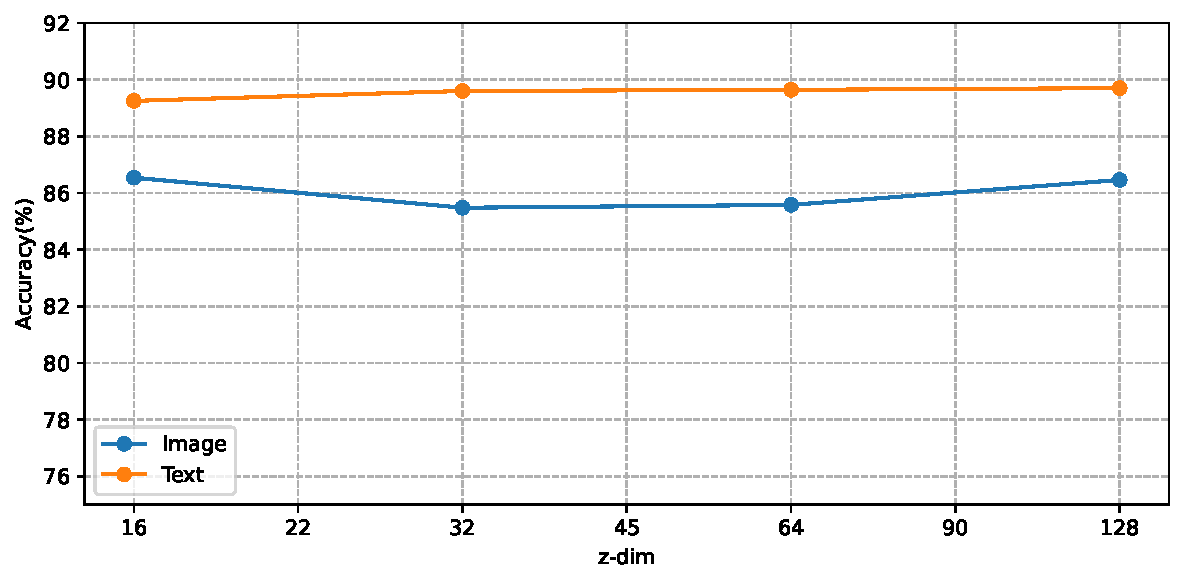
\includegraphics[width=\textwidth]{figs/mega/mega_z.pdf}
\caption{z-dim}
\label{fig:mega_z}
\end{subfigure}
\hspace{0.05\textwidth}
\begin{subfigure}[b]{0.45\textwidth}
\centering
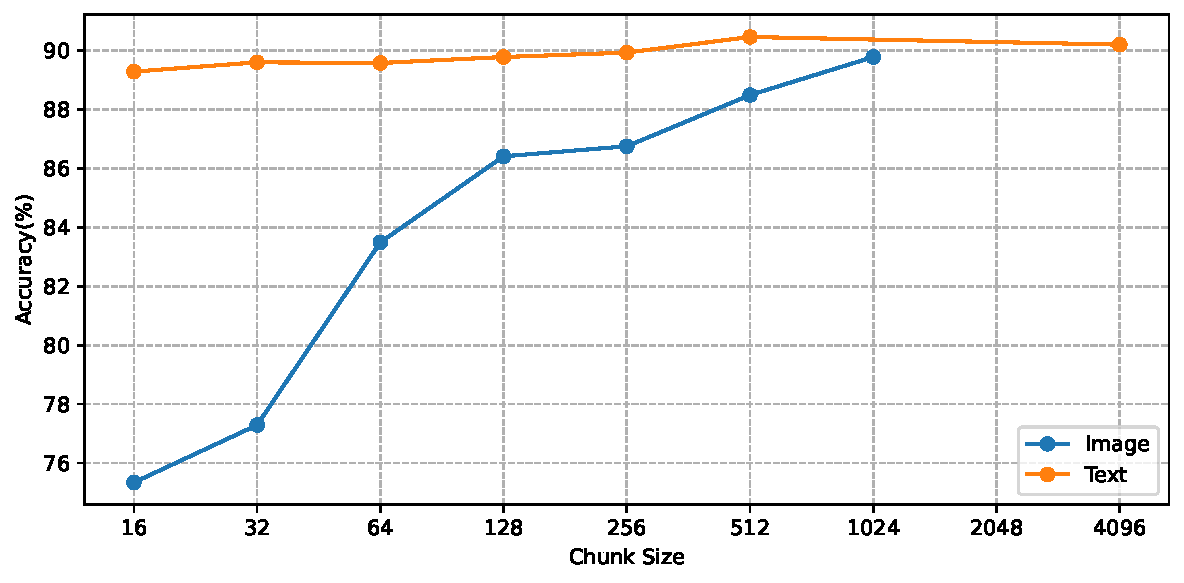
\includegraphics[width=\textwidth]{figs/mega/mega_chunk.pdf}
\caption{chunk size}
\label{fig:mega_chunk}
\end{subfigure}

\caption{MEGA 模型参数对性能的影响}
\label{fig:mega_param}
\end{figure}

\subs{MEGA 方法参数}
对于 MEGA 而言,其提升计算效率的关键在于使用 MEGA-chunk,并尽可能减小分块大小 $c$ 的值。然而过小的 $c$ 导致远距离相关的元素需要更为复杂的传递才能相互作用。这可能使得模型处理远距离信息的能力变弱。因此,我们选取了两个较为有代表性的任务:上下文长度为 4K 的 Text 作为长序列的典型任务,以及上下文长度为 1K 的 Image 作为复杂序列关系的典型任务,来探索部分 MEGA 参数对于建模能力的影响。

首先是MEGA 中序列的高效表征向量 z 的维度。选取维度为$2^4,2^5,2^6,2^7$(即实验中用到的最大值)分别进行训练和推理,结果如图 \ref{fig:mega_z} 所示。可见不同大小的 z 对模型的性能表现几乎没有影响。这很可能是因为 z 维度的特征在计算 Attention 时会被压缩为 1 维的注意力权重,因此即使 16 维的向量也已经携带了充分的信息。换言之,在 Attention计算过程中看似损失的位数可能已经被对z向量的投影过程所补偿。

接下来是 chunk 大小。选用 $c=2^4, 2^5,\cdots,2^{12}$ 分别训练并测量模型的建模效果,结果如图\ref{fig:mega_chunk}所示。实验发现对 Text 任务,跨越多个数量级的 chunk 大小并未对结果产生显著影响,而对于 Image 来说,准确率随 chunk 的增大显著增加。Text 任务中靠相临近的词产生关联即可较为准确的确定情感,此时信息传递效率就并非准确率的瓶颈。而对于 Image 来说,一维距离很远的点可能二维距离很近,因此过小的 chunk 大小显著限制了需要产生相关性的元素之间的相互作用。结合\ref{subsec:lra_perf}中 MEGA-128 在 ListOps 上表现不佳的观察,这很可能说明 MEGA-chunk 在元素具有复杂位置关联的任务上有较大的精度损失。